\section{Why care?}

%\frame{
%	\begin{itemize}[<+->]
%		\item Let's face it.
%		\item I'm stupid.
%		\item I forget things I shouldn't forget.
%		\item I'm lazy. Soooo lazy.
%		\item I don't like to read stuff that I'm not interested in.
%		\item I'd like to live in a world where I can finish tasks without learning tons of unneccessary things.
%		\item And you're like me.
%	\end{itemize}
%}


{ % all template changes are local to this group.
	% 106da1
    \setbeamertemplate{navigation symbols}{}
    \setbeamercolor{background canvas}{bg=bsodcolor}
    \begin{frame}<article:0>[plain]
        \begin{tikzpicture}[remember picture,overlay]
            \node[at=(current page.center)] {
		    \href{run:crash3.mp4?autostart&noprogress}{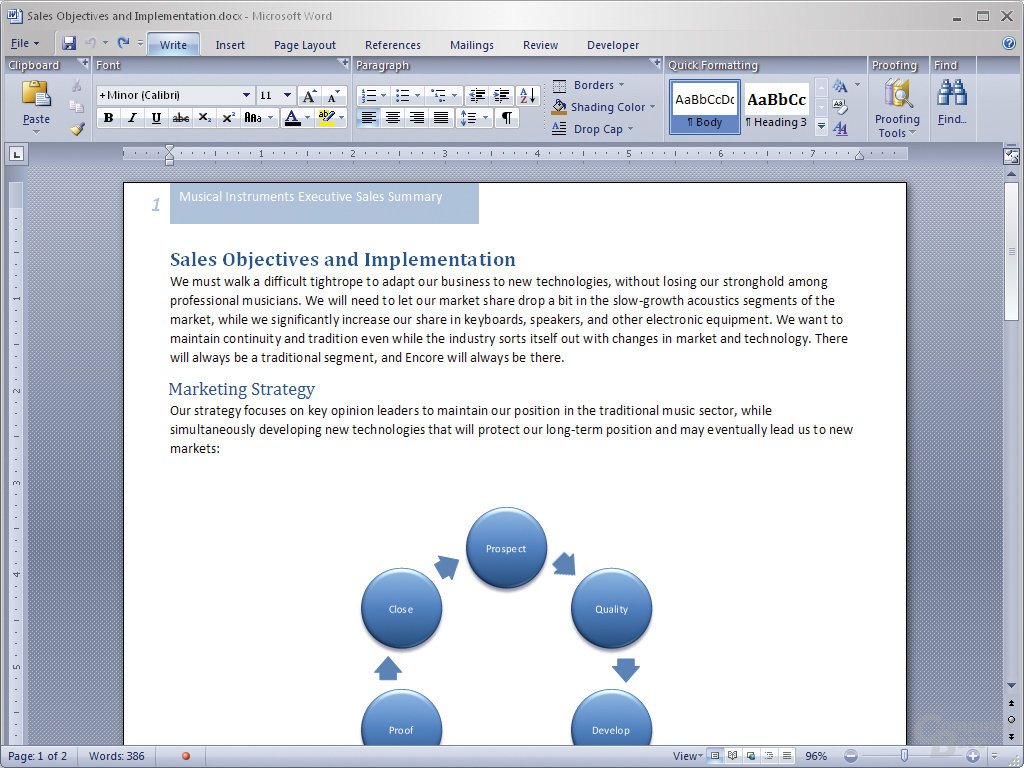
\includegraphics[keepaspectratio,width=\textwidth,height=\textheight]{office12.jpg}}
            };
        \end{tikzpicture}
	\nocite{office12,glitch,wikibsod}
     \end{frame}
}



\note{
	\begin{itemize}
		\item Imagine you're working on an important document and suddenly\dots
		\item Nothing is working anymore, your document probably lost.
		\item You don't perceive this as opportunity to learn more about Computers, how they work and why they fail
		\item It's not an invitation to get more familiar with them. (Even though it absolutely is.)
		\item It's the task that's important, the computer is just a way to solve a task, it should not be the cause of other problems that
			maybe you have no idea how to deal with
	\end{itemize}
}

\frame{
	Let's always remember this on our way to develop better software.

	Good software is that which does \textbf{not} annoy like that. And only good Software gets sold and used. This is why you should care.
}

